\chapter{Antennas}\label{ch:antennas}

In this section different antenna types is analysed and simulated in CST studio. Simple structures such as monopoles and dipoles is not considered since the polarization in the antennas basic form is linear. Even though it is possible to make a crossed dipole array that is circular polarized and have a high gain, but this structure would become large and still not have the opportunity to form the radiation pattern as required. Other structures such as spiral antennas and conical antennas is neither considered since those primarily is used as wideband antennas. This section will investigate the possibility to form the radiation pattern to a field to overcome the requirements from chapter \ref{ch:linkbudget} only.     

\section{Reflector Antennas}

Reflector antennas are used places where a high gain is needed. The reflector antenna do also have a wide bandwith, which all together has made them popular for deep space communication \citep{Imbriale2012}. Although reflector antennas can be made in different types, shapes and configurations, they all essentially consist of a passive reflecting surface illuminated by a smaller primary feed. The basic analysis is done using trigonometry which provides satisfactory result because the diameter of the reflecting surface often is ten times the wavelength. In figure \ref{fig:reflector_types} four main configurations is depicted. (a) is the on-focus parabolic reflector where the feed for the parabolic is placed F distance apart called the focal point. This would leave an area where the feed is placed, where there will be a gap in the coverage. This is omitted in (b) which is the off-axis reflector. This types has no gap in coverage and therefore is often used as radar. The (c) Cassegrain reflector and (d) Gregorian reflector uses both a feed in the middle of the reflector which then uses a second reflector at the focal point to reflect the energy back to the large reflector. Because of the large dimensions a reflector antenna are not suited for low frequencies < 2GHz. Using the equations \ref{eq:para1} to \ref{eq:para4} a design has been made for $f = 10GHz$, $\lambda = 30mm$, $D = 10\lambda = 300mm$, $\theta = 60^{\circ}$. This should give a gain at 30dBi. The design has been simulated in CST studio in figure \ref{fig:para_sim1} and \ref{fig:para_sim2}. The feeding antenna used is a dipole which is an omnidirectional antenna, this causes a loss in efficiency. An ideal reflector should be uniformly illuminated and all power should
be focused on the reflecting surface. The portion of the feed power that does not reach the reflector is referred to
as spillover loss while the ability to uniformly feed the parabola is referred to as illumination efficiency. Since
primary feeds have a tapered radiation pattern, a compromise between spillover losses and illumination
efficiency must be considered to maximize the aperture gain. In the simulation a gain at $G=15dB$ was obtained, this could be optimized using an horn-antenna. 

\begin{figure}[H]
\centering 
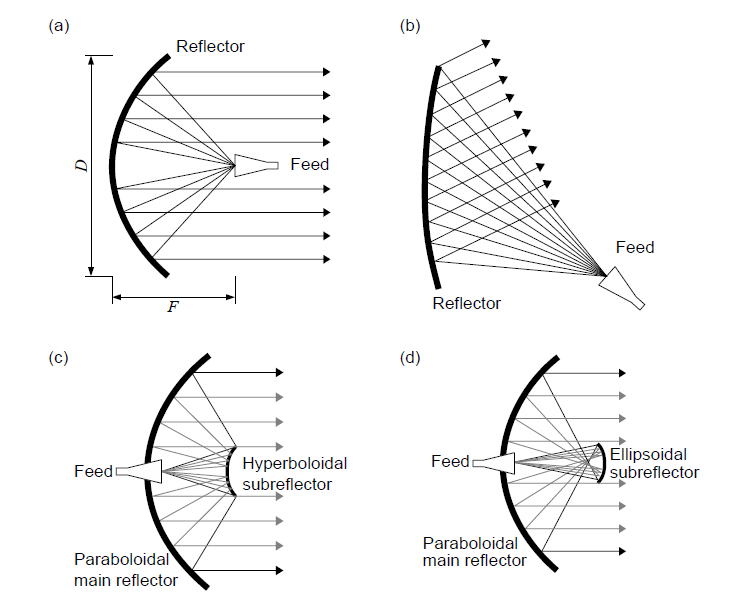
\includegraphics[scale = 0.7]{figures/antennas/reflector/types}
\caption{Reflector antenna configurations: (a) on-focus parabolic reflector; (b) off-axis reflector; (c) Cassegrain reflector; (d) Gregorian reflector \citep{Imbriale2012}}
\label{fig:reflector_types}
\end{figure}

Equation for parabola

\begin{equation}
y=a x^2 , a = \frac{1}{4F}
\end{equation}
\label{eq:para1}

Focal length
\begin{equation}
F=D\frac{1}{4tan(\theta/4)}
\end{equation}
\label{eq:para2}

Length of parabolic segment
\begin{equation}
L=\frac{ln(\sqrt{a^2 D^2 +1}+a D)}{4a}+\frac{D\sqrt{a^2 D^2 +1}}{4}
\end{equation}
\label{eq:para3}

Gain for parabolic reflector

\begin{equation}
G=\eta \frac{4\pi A}{\lambda^2}, A = \frac{\pi D^2}{4}
\end{equation}
\label{eq:para4}

\begin{figure}[H]
\centering 
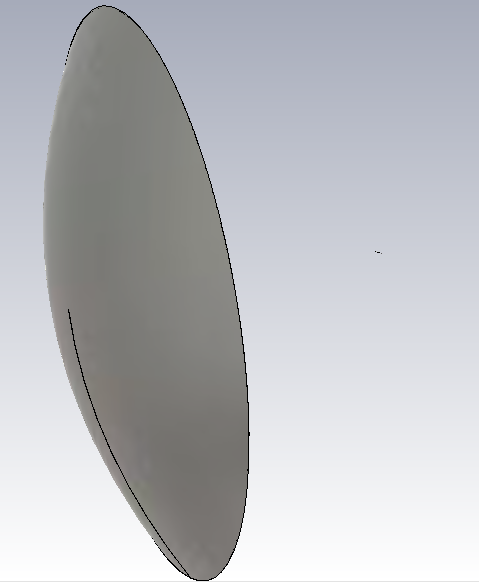
\includegraphics[scale = 0.5]{figures/antennas/reflector/parabola_cst}
\caption{Simulated reflector antenna in CST studio}
\label{fig:para_sim1}
\end{figure}

\begin{figure}[H]
\centering 
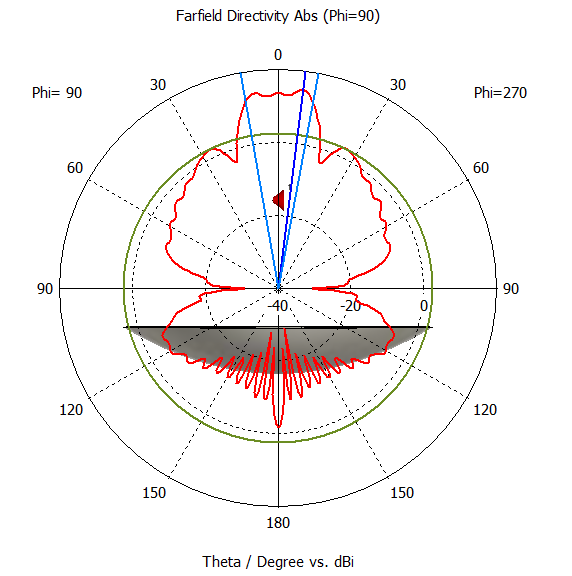
\includegraphics[scale = 0.5]{figures/antennas/reflector/parabola_cst_farfield}
\caption{Farfield of simulated reflector antenna in CST studio}
\label{fig:para_sim2}
\end{figure}



\section{Helical Antennas}
\subsection{Helical antenna with ground plane}

\begin{figure}[H]
\centering 
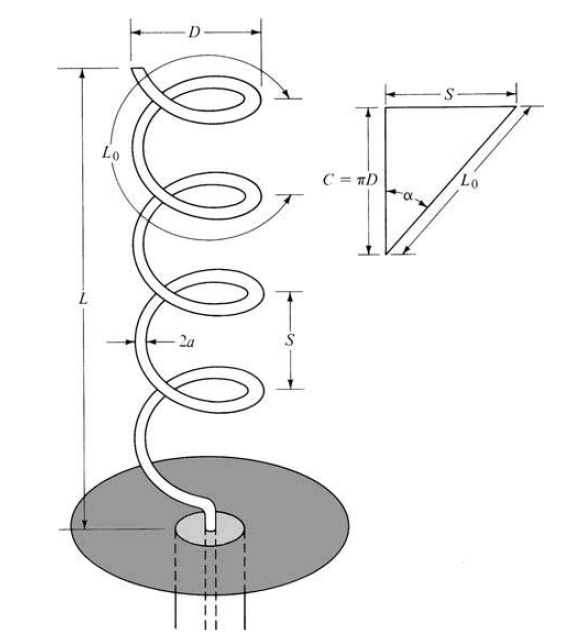
\includegraphics[scale = 0.5]{figures/antennas/helical/helical}
\caption{Helical antenna with ground plane \citep{Balanis2005}}
\label{fig:helical}
\end{figure}

\begin{figure}[H]
\centering 
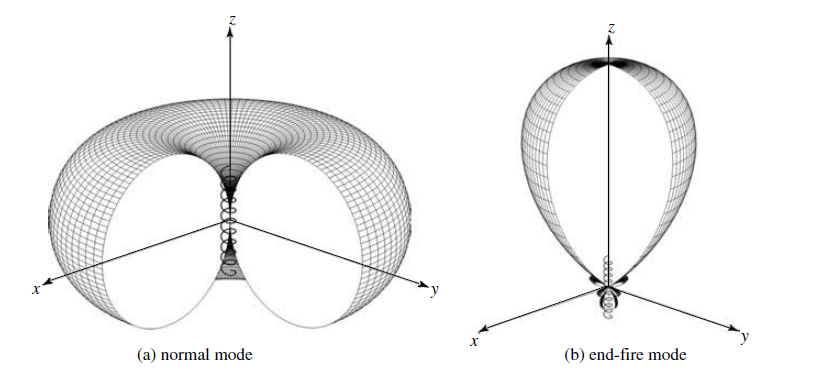
\includegraphics[scale = 0.5]{figures/antennas/helical/modes}
\caption{Farfield for (a) normal mode and (b)end-fire mode in linear scale \citep{Balanis2005}}
\label{fig:helical_modes}
\end{figure}

A helical antenna is a wire wound in form of a screw and is depicted in figure \ref{fig:helical}. The helical antenna consist of N turns, diameter D and spacing between the turns S and circumference is $C = \pi D$ where the total length is $L = NS$. Normally the helical antenna has a circular ground plane with the diameter $G_d = \frac{3\lambda}{4}$. Another important parameter is the pitch angle $\alpha$ which is the angle formed by a line tangent to the helix wire and a plane perpendicular to the helix axis. The pitch angle is defined by   

\begin{equation}
\alpha = tan^{-1}(\frac{S}{\pi D}) = tan^{-1}(\frac{S}{C})
\end{equation} 

The radiation pattern of the antenna can be varied by controlling the size of its
geometrical properties compared to the wavelength. The input impedance is critically
dependent upon the pitch angle and the size of the conducting wire, especially near the
feed point, and it can be adjusted by controlling their values. The general polarization
of the antenna is elliptical. However circular and linear polarizations can be achieved
over different frequency ranges \citep{Balanis2005}. The helical antenna can operate typically in one of two modes which is
the normal (broadside) and the axial (end-fire) mode see figure \ref{fig:helical_modes}. In end-fire mode a circular polarization is archived if the D and S is large fractions of the wavelength. The design criteria is $\frac{3}{4} < C/\lambda < \frac{4}{3}$ where $C = \lambda$ is optimum. $S = \frac{\lambda}{4}$ this gives a pitch angle between $12^o \leq \alpha \leq 14^o $ and a ground plane at least $G_d = \frac{\lambda}{2}$. Formulas for radiation resistance Half Power Beam Width (HPBW) and reflection coefficient is given by equation \ref{eq:heli1} to \ref{eq:heli4}. The formulas has an accuracy about 20\% the formulas are therefore held up with a simulation at $f = 1GHz$.\\

Directivity
\begin{equation}
D =  15N\frac{C^2 S}{\lambda^3} = 12.7dB
\end{equation}  
\label{eq:heli1}

Half Power Beam Width
\begin{equation}
HPBW = \frac{52\lambda^{3/2} }{C\sqrt{NS}} = 46.5^o
\end{equation}  
\label{eq:heli2}

Impedance of antenna 
\begin{equation}
Z_l = 140\frac{C}{\lambda} = 140\Omega
\end{equation} 
\label{eq:heli3}
 
Reflection coefficient 
\begin{equation}
\Gamma = \frac{Z_l+Z_s}{Z_l-Z_s} = -3.2dB
\end{equation}  
\label{eq:heli4}

The simulation results are depicted in figure \ref{fig:helical_cst} to \ref{fig:helical_farfield}. It can be seen that the simulated results corresponds well with the formulas whit in 20\% accuracy. Even though the shape of the radiation pattern can be adjusted by varying the shape of the helix, it it not possible to obtain circular polarization in those "custom" shapes and therefore the helix cannot be used for tracking of ADS-B signals other than in the end-fire mode. 

\begin{figure}[H]
\centering 
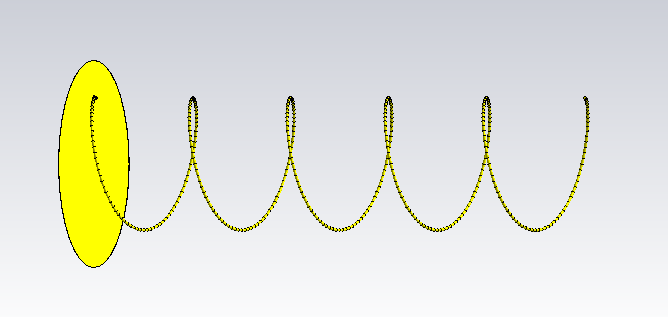
\includegraphics[scale = 0.5]{figures/antennas/helical/helical_cst}
\caption{Simulated helical antenna}
\label{fig:helical_cst}
\end{figure}

\begin{figure}[H]
\centering 
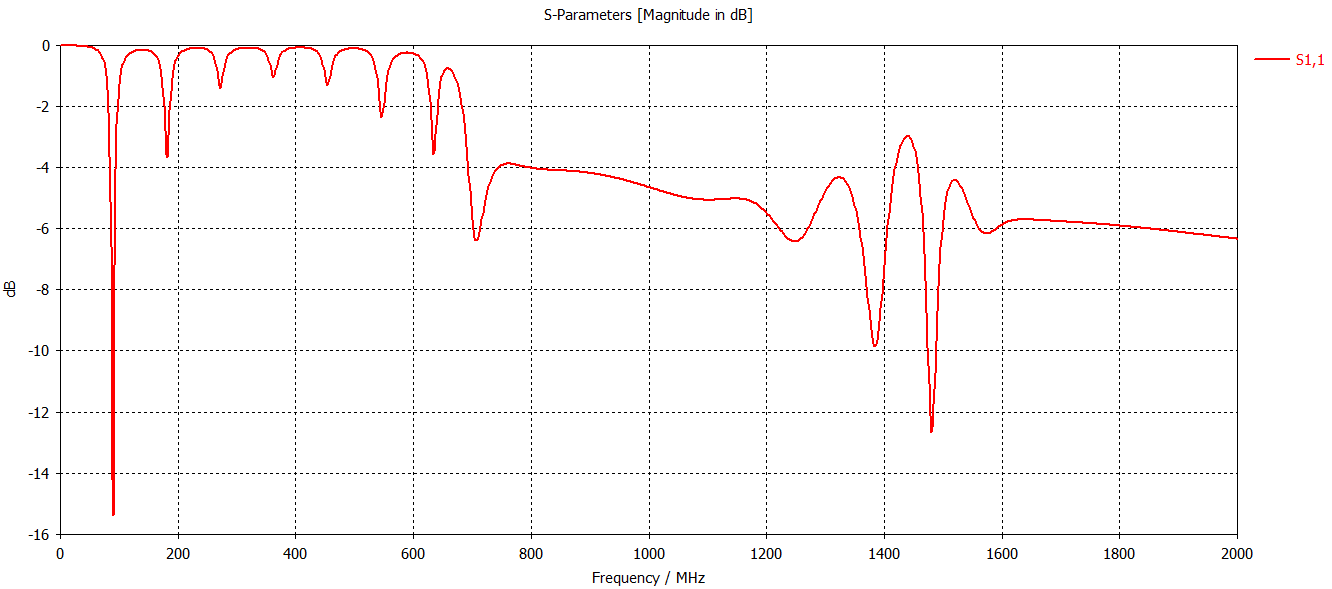
\includegraphics[scale = 0.35]{figures/antennas/helical/helical_cst_s11}
\caption{Reflection coefficient for simulated helical antenna}
\label{fig:helical_s11}
\end{figure}

\begin{figure}[H]
\centering 
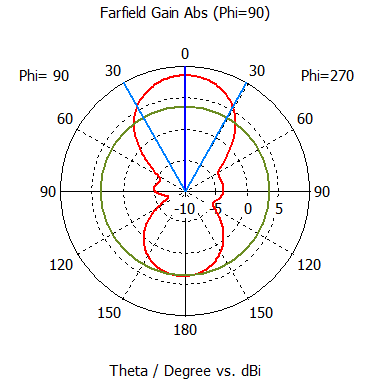
\includegraphics[scale = 0.7]{figures/antennas/helical/helical_cst_farfield}
\caption{Farfield for simulated helical antenna with a maximum gain at 8.5dB and a HPBW at $58.8^o$. This gives a coverage percentage at the earth at 0.5\% }
\label{fig:helical_farfield}
\end{figure}

\subsection{Quadrifilar Helical Antenna}

\begin{figure}[H]
\centering 
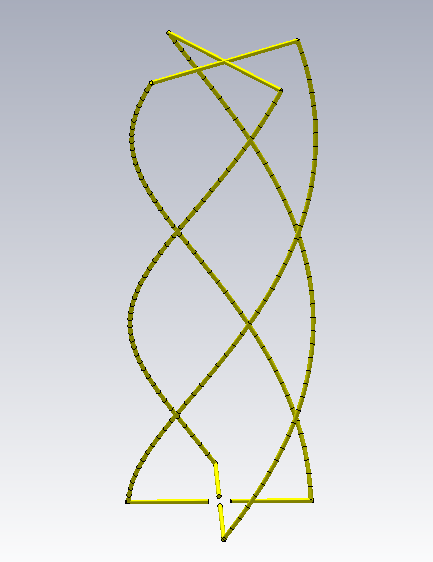
\includegraphics[scale = 0.7]{figures/antennas/qha/qha_6_1mhz}
\caption{QHA with $N=0.6$, $D=80mm$,$L=\frac{\lambda}{2}-D\cdot 0.75$, $f=1GHz$}
\label{fig:QHA1}
\end{figure}

The Quadrifilar Helical Antenna (QHA) (see figure \ref{fig:QHA1}) is an resonant antenna which is typically feed by two ports with a $90^\circ$ phase difference. The antenna has a circular polarization and the size is often smaller than a normal helical antenna. Typically the length of each arm is an integral multiple of the quarter-wavelength. The end of the helix
is open when the integer is odd, while short when the integer is
even \citep{Bai2014}. Despite the typically design the turn ratio, radius, length and feeding topology will affect the radiation pattern and polarization. 
\newline
\newline
An QHA has been build and simulated in CST studio. The dimensions are $D=80mm$,$L=\frac{\lambda}{2}-D\cdot 2$, $N=0.6$ at the frequency $f=122.5MHz$ and $\lambda = 2450mm$ with the wire diameter $Wd = 2mm$. The length is calculated so there is a half wavelength for the current flow between the negative and positive side of a port. The feeding is done using two discrete ports as shoved in figure \ref{fig:QHA2}.  

\begin{figure}[H]
\centering 
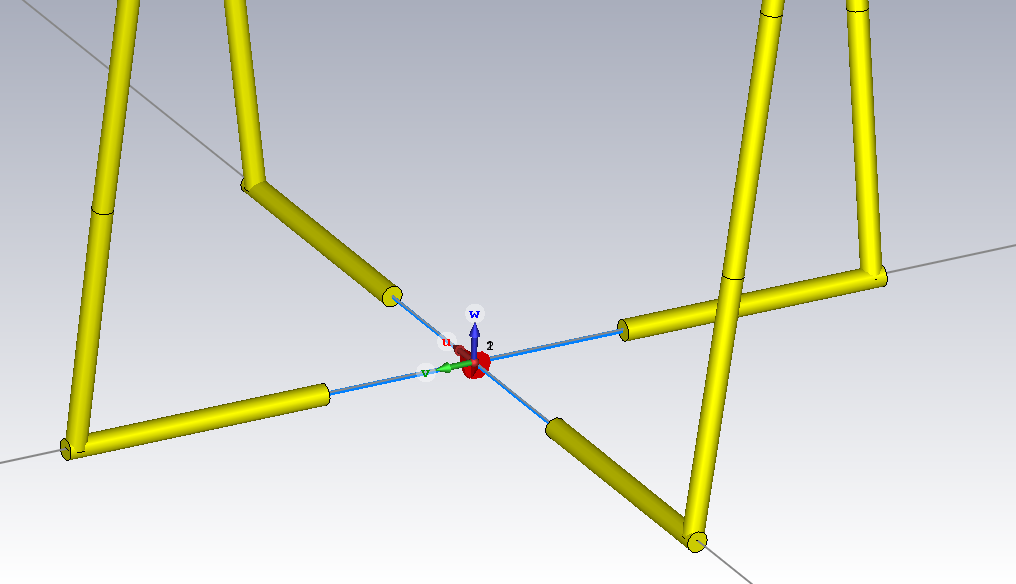
\includegraphics[scale = 0.4]{figures/antennas/qha/qha_6_feeding}
\caption{Feeding of the QHA for 122.5MHz using discrete ports}
\label{fig:QHA2}
\end{figure}
 
The QHA has been simulated and the results shows, that the antenna is resonating at 131MHz even thou the S11 parameter at this frequency is only -2dB, see figure \ref{fig:QHA_S11}. The small difference in frequency due to the calculations is caused by the gap between the ports in the bottom and the extra length caused by the turn of N. It can be seen that the antenna also radiates at multiply of the first resonant frequency and that the lowest return-loss is obtained at 4 times the frequency which gives 519MHz. The farfields for the frequencies 131,262,393 and 519MHz are shown in figure \ref{fig:QHA_ff_131}, \ref{fig:QHA_ff_262}, \ref{fig:QHA_ff_393} and \ref{fig:QHA_ff_519}, where port 1 is fed with a positive phase at $90^\circ$. It is seen that the farfield not surprisingly changes with the frequency and that a higher frequency will result in side lobes. This could be an advantage to overcome the requirement from figure \ref{fig:sat_farfield} but unfortunately the polarization becomes linear in the angle of the sidelobes which then makes this option unuseful.        

\begin{figure}[H]
\centering 
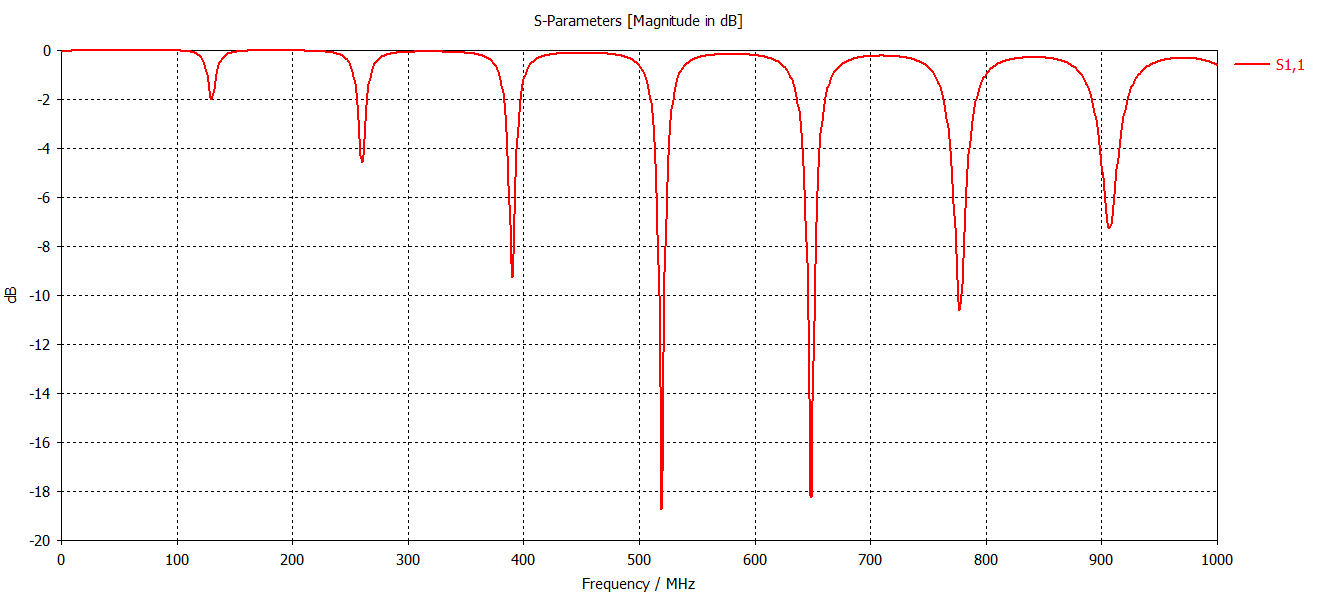
\includegraphics[scale = 0.4]{figures/antennas/qha/qha_6_S11}
\caption{S11 parameter of the QHA for 122.5MHz}
\label{fig:QHA_S11}
\end{figure}

\begin{figure}[H]
  \centering
  \begin{minipage}[b]{0.5\textwidth}
	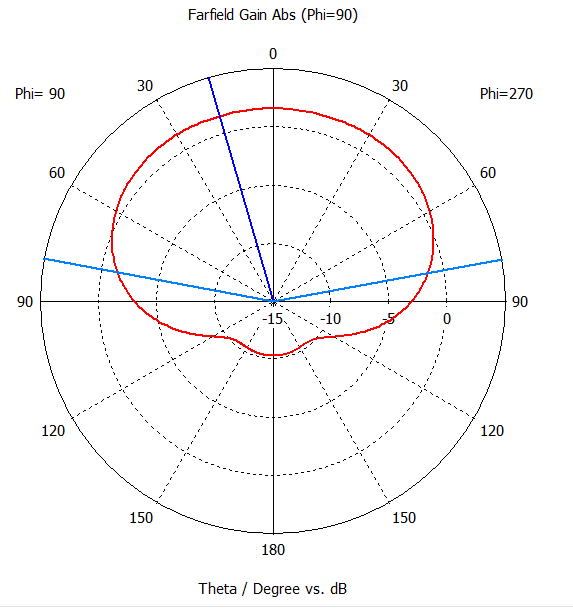
\includegraphics[scale = 0.4]{figures/antennas/qha/qha_6_ff_131}
	\caption{Simulated farfield at 131MHz}	
    \label{fig:QHA_ff_131}
  \end{minipage}
  \hfill
  \begin{minipage}[b]{0.4\textwidth}
	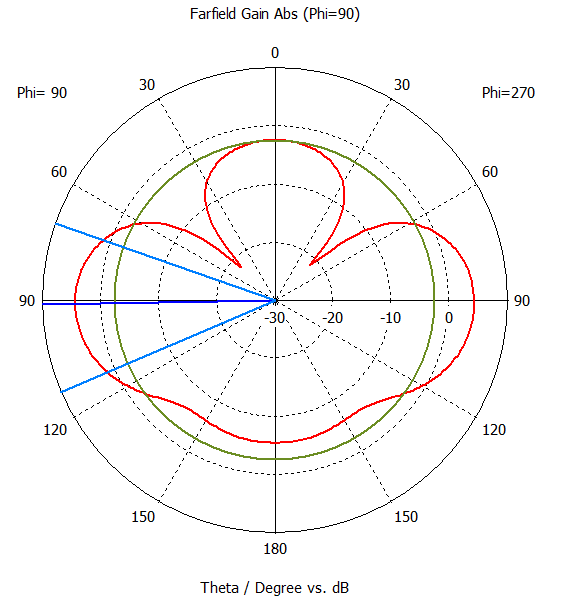
\includegraphics[scale = 0.4]{figures/antennas/qha/qha_6_ff_262}
	\caption{Simulated farfield at 262MHz}
    \label{fig:QHA_ff_262}
  \end{minipage}
\end{figure}


\begin{figure}[H]
  \centering
  \begin{minipage}[b]{0.5\textwidth}
	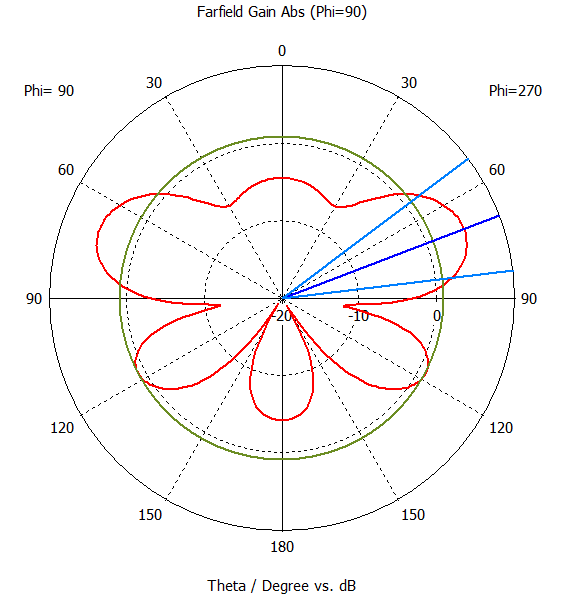
\includegraphics[scale = 0.4]{figures/antennas/qha/qha_6_ff_393}
	\caption{Simulated farfield at 393MHz}
    \label{fig:QHA_ff_393}
  \end{minipage}
  \hfill
  \begin{minipage}[b]{0.4\textwidth}
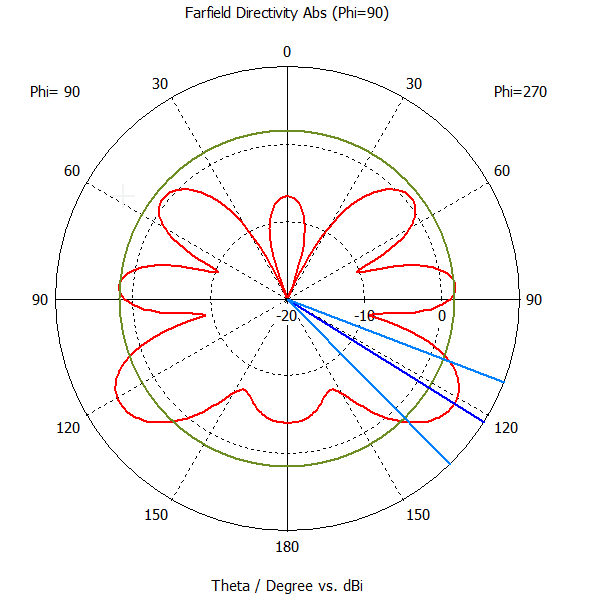
\includegraphics[scale = 0.4]{figures/antennas/qha/qha_6_ff_519}
\caption{Simulated farfield at 519MHz}
    \label{fig:QHA_ff_519}
  \end{minipage}
\end{figure}

%%%%%%%%%%%%%%%%%%%%%%%%%%%%%%%%%%%%%%%%%%%%%%%%%% Axial Ratio
\begin{figure}[H]
  \centering
  \begin{minipage}[b]{0.5\textwidth}
	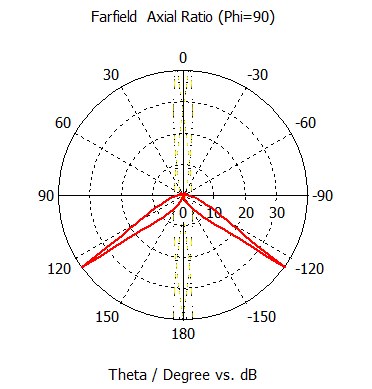
\includegraphics[scale = 0.6]{figures/antennas/qha/qha_6_ff_131_AR}
	\caption{Simulated Axial Ratio at 131MHz}	
    \label{fig:QHA_ff_131_AR}
  \end{minipage}
  \hfill
  \begin{minipage}[b]{0.4 \textwidth}
	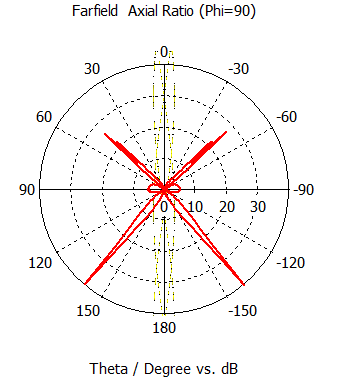
\includegraphics[scale = 0.6]{figures/antennas/qha/qha_6_ff_262_AR}
	\caption{Simulated Axial Ratio at 262MHz}
    \label{fig:QHA_ff_262_AR}
  \end{minipage}
\end{figure}


\begin{figure}[H]
  \centering
  \begin{minipage}[b]{0.5\textwidth}
	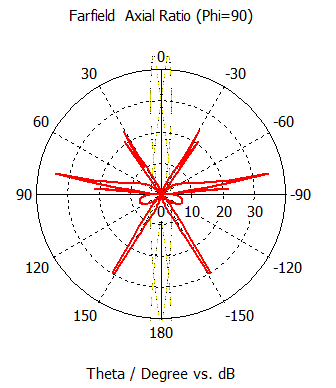
\includegraphics[scale = 0.6]{figures/antennas/qha/qha_6_ff_393_AR}
	\caption{Simulated Axial Ratio at 393MHz}
    \label{fig:QHA_ff_393_AR}
  \end{minipage}
  \hfill
  \begin{minipage}[b]{0.4\textwidth}
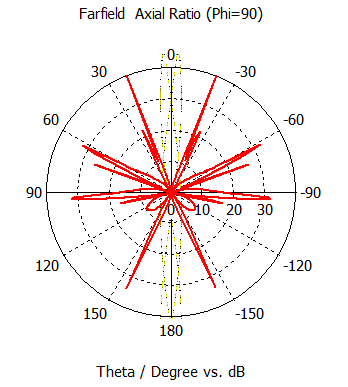
\includegraphics[scale = 0.6]{figures/antennas/qha/qha_6_ff_519_AR}
\caption{Simulated Axial Ratio at 519MHz}
    \label{fig:QHA_ff_519_AR}
  \end{minipage}
\end{figure}

%%%%%%%%%%%%%%%%%%%%%%%%%%%%%%%%%%%%%%%%%%%%%%%%%%%%%%%%%%%%%%%%%%%%%%%%%%%%%%%%%%%%% Feeding %%%%%%%%%%%%%%%%%%%%%%%%%%%%%%%%%%%%%%%%%%%%%
\subsubsection{Feeding methods}
In figure \ref{fig:QHA2} the feeding of the QHA is done using two discrete ports. When port 1 is fed with a positive phase at $90^\circ$ the QHA will have it's maximum radiation in the forward direction. If the port instead is fed with a negative phase at $90^\circ$ then the QHA will have it's maximum radiation in the backward direction. Other phases will result in non-uniform radiation patterns with one ore more peaks in the azimuth axis. It is easy to believe that it is possible to connect two of the arms of the QHA to a common ground and feed the one port with a phase difference at $90^\circ$ using a $1/4 \lambda $ transmission-line and the other directly from the source depicted in figure \ref{fig:QHA_common}. But this will not work since the geometry of the QHA will change from an electrically perspective. The shortening of the two grounds will affect the flow of the current resulting of only a pattern difference of $45^\circ$ in the farfield which then makes it impossible to archive a omnidirectional radiation pattern and circular polarization. To overcome this is has been shown in \citep{Bai2014} that it is possible to use a feeding network consisting of one second-iteration Moore $180^\circ$ hybrid coupler and two second-iteration Sierpinski $90^\circ$ hybrid couplers. It has also been showen in \citep{Yang2014} that a broadband feed network can be done using an wilkinson powerdivider and broadband $90^\circ$ phase shifters.     

\begin{figure}[H]
\centering 
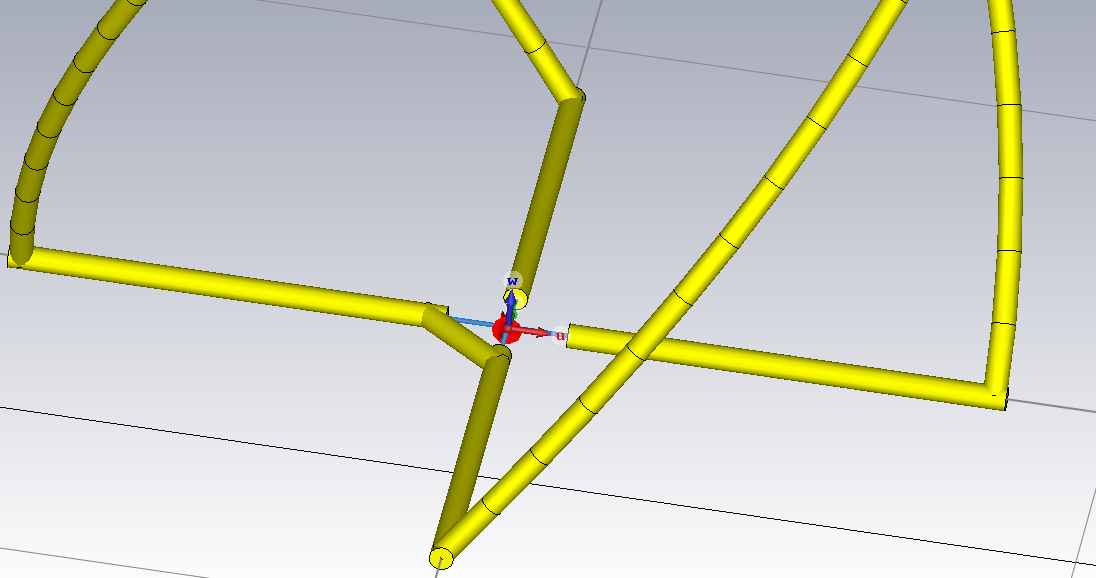
\includegraphics[scale = 0.3]{figures/antennas/qha/qha_6_common_gnd}
\caption{Common GND for the QHA}
\label{fig:QHA_common}
\end{figure}

%%%%%%%%%%%%%%%%%%%%%%%%%%%%%%%%%%%%%%%%%%%%%%%%%%%%%%%%%%%%%%%%%%%%%%%%%%%%%%%%%%%%% wideband %%%%%%%%%%%%%%%%%%%%%%%%%%%%%%%%%%%%%%%%%%%%%
\subsubsection{Wideband QHA}
As shown previously a QHA in its basic form radiates only at a narrow frequency band. For the S-parameters in figure \ref{fig:QHA_S11} it is seen that at 131MHz the return loss is about -2dB which results in an efficiency at only -5dB. This can be improved using a match network, but the antenna still needs to be a radiating element and therefore the matching can only improve the return-loss and not the bandwidth \citep{Iyver2010}. Therefore some modifications needs to be done at the QHA to improve the bandwidth. One method is to make the bifilar arms of the QHA in diffrent lengths so one arm is longer than the resonant frequency and the other shorter as depicted in figure \ref{fig:WB_QHA}. The feeding is done by shortening the feeds as in figure \ref{fig:WB_QHA_feed} and feed with a $1/4\lambda$ coax cable as balun. Because the feeding is done this way the farfield will not be omnidirectional and is skewed in one direction as depicted in figure \ref{fig:WB_QHA_ff} but still useful in some applications. The S-parameter in figure \ref{fig:WB_QHA_spar} shows a bandwidth at 10\% which is limited by the $1/4\lambda$ balun. This could be improved, but the farfield will then change and the improvements will be doubtful.       


\begin{figure}[H]
  \centering
  \begin{minipage}[b]{0.5\textwidth}
    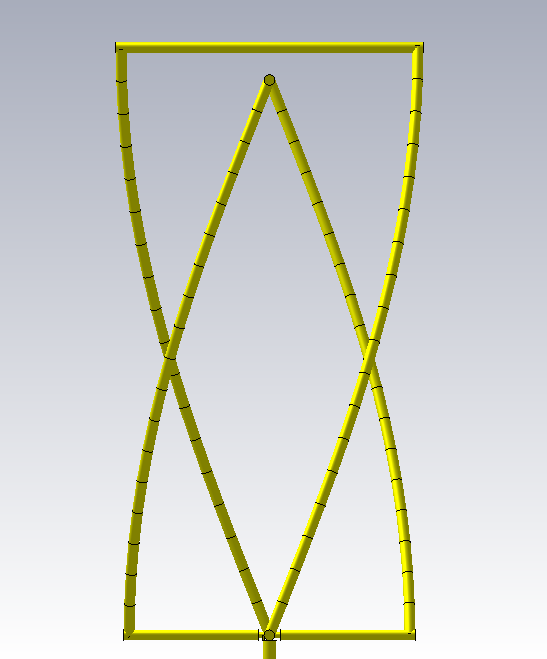
\includegraphics[scale = 0.3]{figures/antennas/qha/wideband}
    \caption{Wideband QHA with dimentions $f = 1GHz$, $\lambda = 300mm$, $R1 = \lambda 0.091$, $ L = \lambda 0.36$, $R2 = \lambda 0.086$, $ L = \lambda 0.34$}
    \label{fig:WB_QHA}
  \end{minipage}
  \hfill
  \begin{minipage}[b]{0.4\textwidth}
	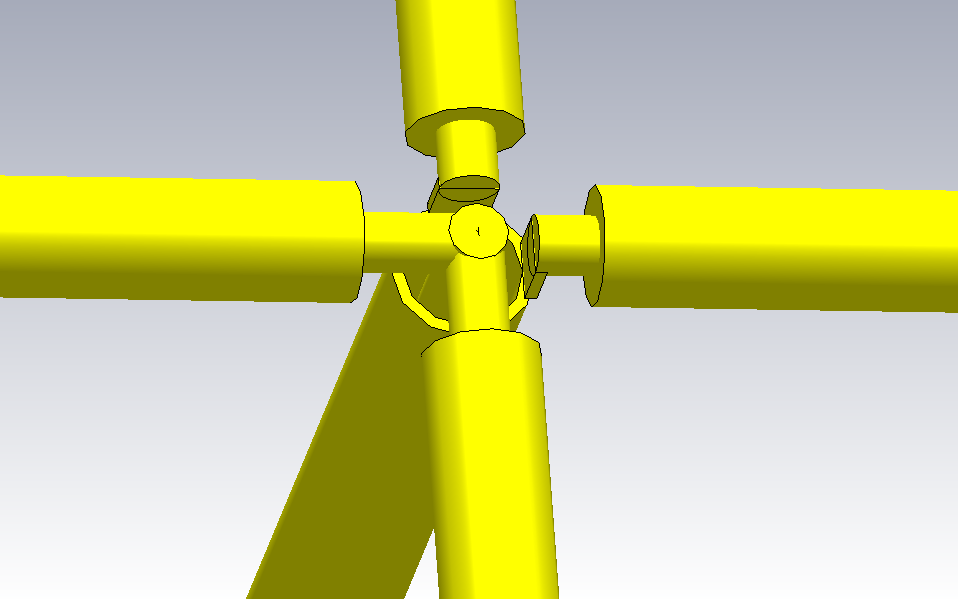
\includegraphics[scale = 0.3]{figures/antennas/qha/wideband_feeding}
    \caption{Feeding for the wideband QHA}
    \label{fig:WB_QHA_feed}
  \end{minipage}
\end{figure}

\begin{figure}[H]
\centering 
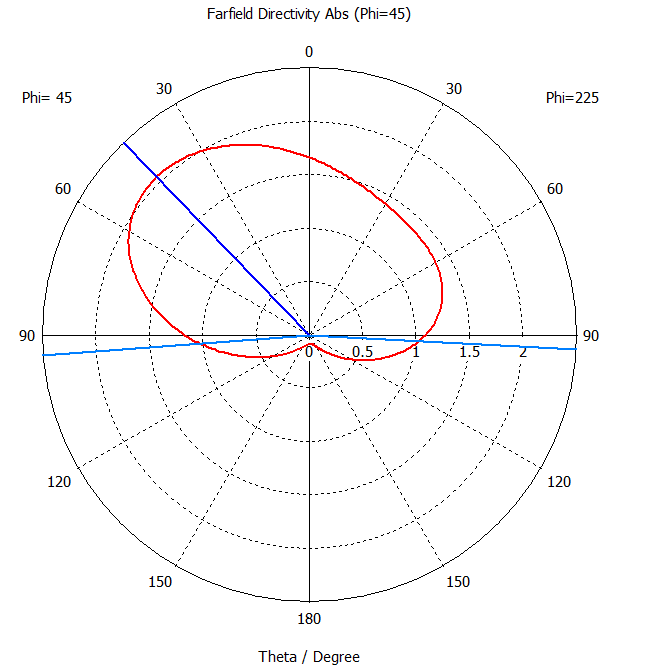
\includegraphics[scale = 0.4]{figures/antennas/qha/wideband_ff}
\caption{Farfield for the wide band QHA in linear scale}
\label{fig:WB_QHA_ff}
\end{figure}   

\begin{figure}[H]
\centering 
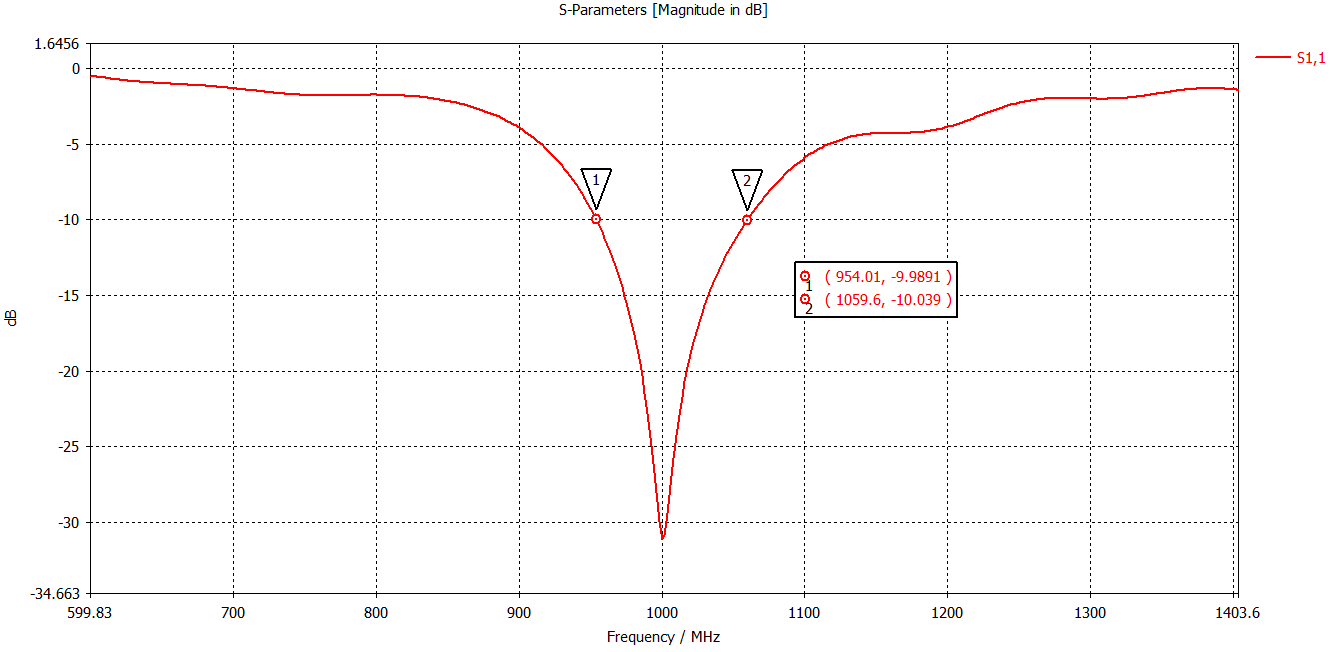
\includegraphics[scale = 0.4]{figures/antennas/qha/wideband_spar}
\caption{S-parameters for the wideband QHA shows a bandwidth at 10\%}
\label{fig:WB_QHA_spar}
\end{figure} 

%%%%%%%%%%%%%%%%%%%%%%%%%%%%%%%%%%%%%%%%%%%%%%%%%%%%%%%%%%%%%%%%%%%%%%%%%%%%%%%%%%%%% wideband %%%%%%%%%%%%%%%%%%%%%%%%%%%%%%%%%%%%%%%%%%%%%
\subsubsection{Multiband QHA}
Another configuration of the QHA is the Multiband QHA \citep{Bai2014} which can be build up on several narrowband or wideband QHA's inside each other as depicted in figure \ref{fig:TB_QHA}. This configuration allows several frequency bands to be covered since several QHA's can be build inside each other. The consequence is though a heavy and complex design which may also needs a complicated feeding network or several ports for each frequency.  

\begin{figure}[H]
\centering 
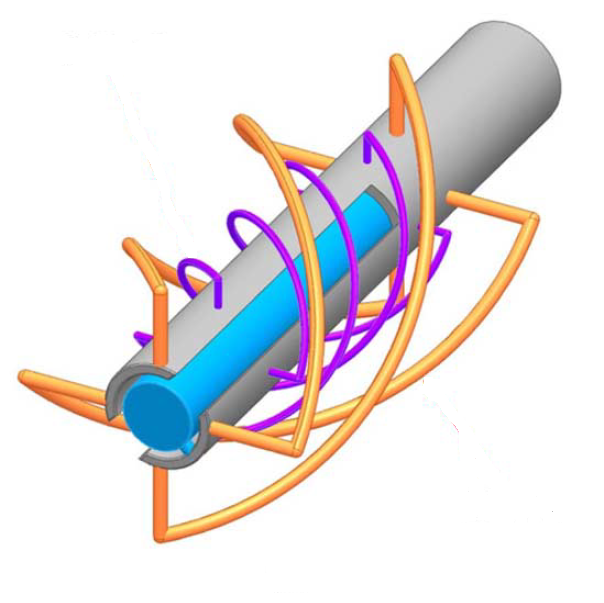
\includegraphics[scale = 0.5]{figures/antennas/qha/dual_band}
\caption{Dual band QHA using two single QHA's \citep{Bai2014}}
\label{fig:TB_QHA}
\end{figure} 



%%%%%%%%%%%%%%%%%%%%%%%%%%%%%%%%%%%%%%%%%%%%%%%%%%%%%%%%%%%%%%%%%%%%%%%%%%%%%%%%%%%%%%%%%%%%%%%%%%%%%%%%%%%%%%%%%%%%%%%%%%%%%%%%%% 


\section{Truncated Spherical Helical Antenna}
The Bifilar Truncated Spherical Helical Antenna (BTSHA) is a modification of the normal Spherical Helical Antenna (SHA) whos geometry is described by equation \ref{eq:SHA1} to \ref{eq:SHA3} where N is number of turns of the wire. The BTSHA is made upon two half's of the SHA which then is turned $180^\circ$ to connect to each other. See figure \ref{fig:SHA1}.  

\begin{equation}\label{eq:SHA1}
r = a
\end{equation}

\begin{equation}\label{eq:SHA2}
\theta = cos^{-1}(\frac{\phi}{N\pi}-1)
\end{equation}

\begin{equation}\label{eq:SHA3}
0<=\phi<=2\pi N
\end{equation}

The BTSHA can be fed different ways using bottom feeding, side feeding or top feeding. One advantage using top feeding is that it can be fed using a "monopole" that will make a field inside the BTSHA together with the current flowing in opposite direction which makes it able to radiate in axial-null mode because of the symmetry. See figure \ref{eq:SHA2}. This makes it possible to archive better gain in the side direction as wanted for a satellite antenna for reception of ADS-B. Another advantage is the compact size compared to a conventional helical antenna. An important feature of this structure is that the angle of the cone can be adjusted by moving the height of the ground-plane. If the cone shall become broader the ground plane can be moved backward and if the cone is wanted narrower then the ground plane can be formed as an reflector. Unfortunately the structure has a lack of gain in the center. Simulations has shown that the number of the wire turns has only little effect on the S-parameter and radiation pattern. A simulation has been made with the dimension $a=2.86\lambda$, see figure \ref{fig:SHA_ff1}. It is stated in \citep{Clark2003} that the radiation pattern for this configuration should be omnidirectional. This has been shown not to be true and there is only two main-beams. The polarization is overall circular but with linear polarization in the direction of the two main-beams.    

\begin{figure}[H]
\centering 
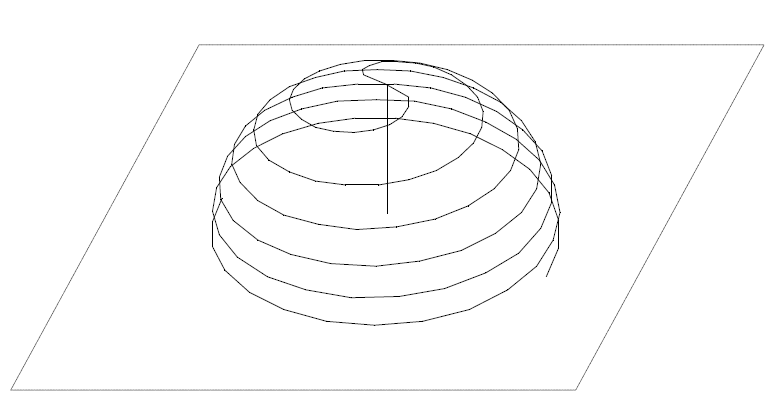
\includegraphics[scale = 0.5]{figures/antennas/hemispherical/hemispherical1}
\caption{Bifilar Truncated Spherical Helical Antenna \citep{Clark2003}}
\label{fig:SHA1}
\end{figure} 

\begin{figure}[H]
\centering 
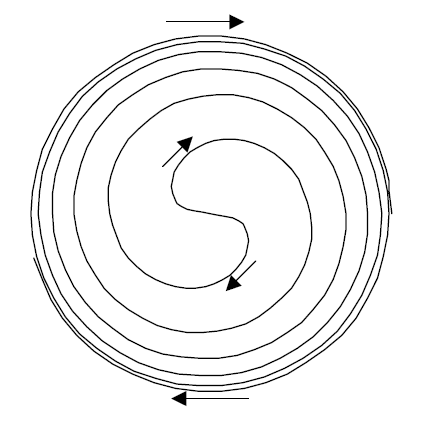
\includegraphics[scale = 0.5]{figures/antennas/hemispherical/hemispherical_currentflow}
\caption{Currentflow of the BTSHA \citep{Clark2003}}
\label{fig:SHA2}
\end{figure} 


\begin{figure}[H]
\centering 
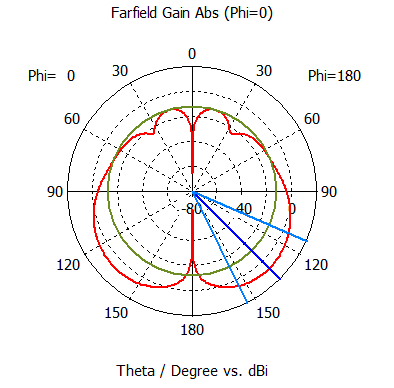
\includegraphics[scale = 0.7]{figures/antennas/hemispherical/hemispherical_farfield1}
\caption{Farfield of a simulated BTSHA with $a=2.86\lambda$ and $N=1.5$. Maximal gain is 7.1dB. Be aware that the strucure at only this farfield is pointing at $180^\circ$}
\label{fig:SHA_ff1}
\end{figure} 

Another simulation has shown to have a more omnidirectional radiation pattern, which uses four arms instead of two (QTSHA) with a rotation of $90^\circ$ each. Futher the structure is streched in the Z-direction by a factor of two. But still this structure has a lack of gain in the center. To overcome this problem simulations has shown that it is rather difficult to make a change to the structure that will increase the gain in the middle. The best solution to this problem is to change the feed point, see figure \ref{fig:SHA_feed}. The feeding point has been simulated for various points and a feeding point at $0.06\lambda$ from the top has shown to be the best. See figure \ref{fig:SHA_ff3}. Unfortunately this asymmetry makes the polarization of the antenna more linear which then makes this option a bad decision.     

\begin{figure}[H]
\centering 
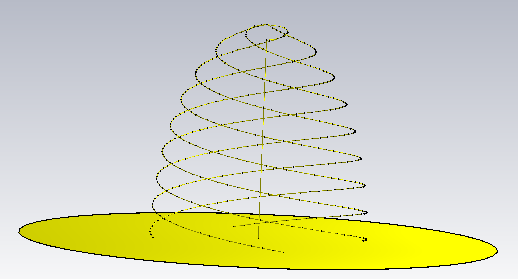
\includegraphics[scale = 0.7]{figures/antennas/hemispherical/hemispherical2}
\caption{Stretched Quadrifilar Truncated Spherical Helical Antenna}
\label{fig:SH32}
\end{figure} 

\begin{figure}[H]
\centering 
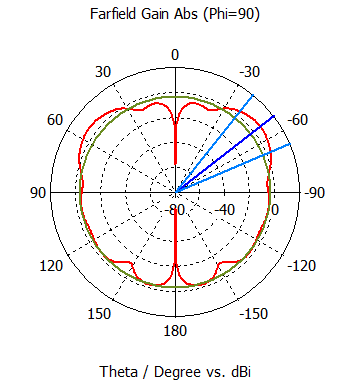
\includegraphics[scale = 0.7]{figures/antennas/hemispherical/hemispherical_farfield2}
\caption{Farfield of a simulated QTSHA with $a=2.86\lambda$ and $N=1.5$. Maximal gain is 5.9dB}
\label{fig:SHA_ff2}
\end{figure} 

\begin{figure}[H]
\centering 
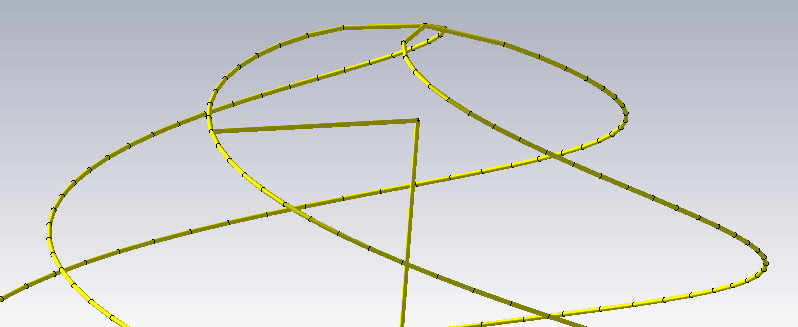
\includegraphics[scale = 0.5]{figures/antennas/hemispherical/hemispherical_feed}
\caption{Position of the changed feeding point}
\label{fig:SHA_feed}
\end{figure}

\begin{figure}[H]
\centering 
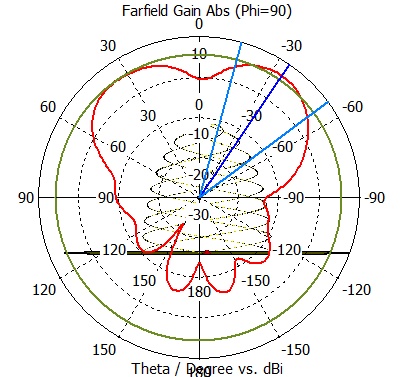
\includegraphics[scale = 0.7]{figures/antennas/hemispherical/hemispherical_farfield3}
\caption{Farfield of a simulated QTSHA with $a=2.86\lambda$ and $N=1.5$. The figure is fully omnidirectional.}
\label{fig:SHA_ff3}
\end{figure}  

\begin{figure}[H]
\centering 
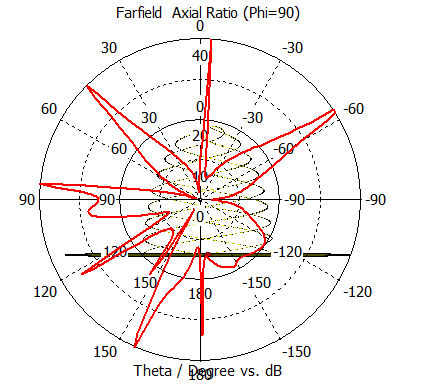
\includegraphics[scale = 0.7]{figures/antennas/hemispherical/hemispherical_farfield3_AR}
\caption{Axial ratio of the simulates antenna shows that this is not a circular polarized antenna}
\label{fig:SHA_ff3_AR}
\end{figure} 












    



   